\section{Waffle}
\label{sec:3-instr}

% Done: The key idea is that I should talk about my solution to the program with more details.
% Done: I have explained that there is another way of resolving the problem.
% Now it's time to explain what is the difference in the guidance defined in Waffle
% Definitions?!:
% Resource complexity, Overall resource complexity (ORC), Elites, Visitors
% OR: Shared memory, instrumentation, fuzzing

% How does the new features solve the problem?
% ! CHANGE Instruction to Machine Instruction

% Tasks
% -T1: Explain the way AFL works
% -T2: Explain an overview of the additional properties added to AFL by Waffle
% Keywords 
% -K1: exploration vs exploitation
% -K2: performance-guided fuzzing vs coverage-guided fuzzing

\begin{figure}[!t]
  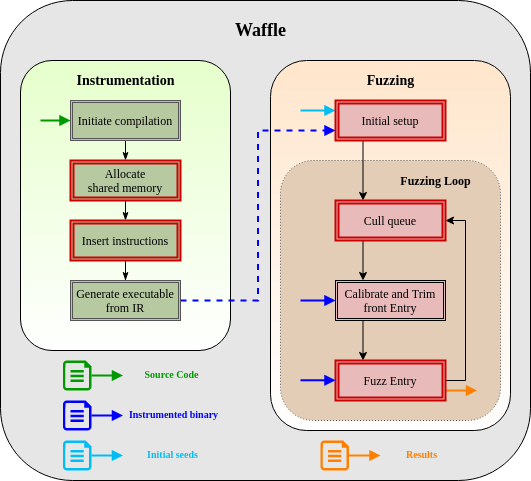
\includegraphics[width=0.8\textwidth]{Chapter3/waffle-proc.png}
  \centering
  \caption{Fuzzing phases of Waffle. The red rectangles specify the changed components.}
  \label{fig:waffle-phases}
\end{figure}

The exponential search space for different inputs with a specific behavior, such as a crash or hang, is approached by evolutionary algorithms of AFL to investigate the possible solutions for producing such events. AFL leverages on code coverage, file size, and execution time to guide the Genetic Algorithm to maintain the cases which discover more regions of the code, in a fast fasion. Waffle \textit{exploits} the coverage-guided findings for more resource usages. The key idea is to measure the performance in an execution, and provide this information in fuzzing phase to generate resource exhaustive inputs. 

% -T: Explain the waffle-proc.png

As illustrated in Figure \ref{fig:waffle-phases}, Waffle has major modifications on AFL in instrumentation phase (shared memory allocation and instructions insertion) and fuzzing phase. The shared memory is designed to be capable of storing the \textit{resource complexity} of an execution. Waffle also extends AFL's Coverage Pass to collect performance features as well. In the fuzzing phase, Waffle evaluates the code coverage and resource usage of the execution, and based on this information culls the queue of entries to consider the new performance measurements. In the following sections we inspect the changes and assess the effectiveness of the work.

\subsection{Resource complexity of execution}

% ?   #########################################################################
% -T: What the resource complexity is and how it is measured

To address resource usage of an execution, we estimate the engaged resources in an execution. Waffle does not analyse the source code for finding the resource complexities, such as time and space complexity, however, it records the instructions responsible for resource consumptions. For instance, an instruction such as \texttt{memcpy} takes CPU usage (and time) for its execution, and may access the program's available memory. To bring in the involved instructions in a complete run of a program, Waffle selects a set of instructions and monitors the program's execution of such instructions. The accumulation of the executed instructions is then stored partially in the shared memory.

% ?   #########################################################################
% -T1: Estimated Resource Usage

We define the \textbf{Estimated Resource Usage} (shortened to ERU) of an application for \textit{an estimation of the resources required to execute a program}. To evaluate the ERU of a program in a concrete execution, each instruction which uses the \textit{engaging resources} should be monitored. For instance, an instruction such as \texttt{memcpy} takes CPU usage for its execution, and may access the program's available memory.  

% ?   #########################################################################
% -T1: How waffle uses the ERU through entire fuzzing chain

Waffle replicates AFL's coverage-discovery techniques with modifications to calculate and leverage ERU for performance-guidance. Waffle selects a set of instructions and counts their executions to get ERU. The ERU is then stored in an array of the same size as the AFL's coverage map, and for each hit on the coverage map, Waffle changes the same index of it's performance array. As a result, the hitmaps of both of the arrays are the same, and they both can represent the code-coverage; each index is found based on the taken edge of the CFG. Later, in the fuzzing phase, Waffle uses ERU to choose the \textit{favored} entries of queue. In AFL, a favored entry is relates to the input which brings something new, that is, a better code coverage or a faster execution. Instead, Waffle finds the \textit{favor} in any entry which is either AFL-guided or Waffle-guided; a better code coverage or a more exhaustive execution.

% !     Subsection 1: Instrumentation
\subsection{Instrumentation}
\label{subsec:inst}

% ?   #########################################################################
% -T1: Generally define and explain the added and modified modules in Instrumentation

\begin{lstlisting}[language=C++,style=CodeStyle,label={lst:hash},caption={Select element and update in shared\_mem}]
  counter = lg(count_instructions())
  cur_location = <COMPILE_TIME_RANDOM>;
  edge = cur_location ^ prev_location;

  cov_shared_mem[edge]++;
  per_shared_mem[edge]+=counter;

  prev_location = cur_location >> 1;
\end{lstlisting}

Waffle starts its instrumentation by specifying the shared memory region. Waffle maintains an array of 4bytes integers for tracking the ERU of each basic block. This array's length is the same as the AFL's shared array, and as a result, the Waffle's array requires 4x more memory space (Listing \ref{lst:wafl-rt}). This array is set to hold the counts of the edges according to the paths explored. When the initial setups are completed, the next instrumentation step, taking the Module Pass starts.
  
\lstinputlisting[language=C,style=CodeStyle,float=tb,label={lst:wafl-rt},caption={LLVM instrumentation initialization - \texttt{\_\_wafl\_area\_ptr} is the region that is allocated for instruction counters}]{Codes/Chapter3/waffle-llvm-rt.o.c}  

% ?   #########################################################################
% -T1: Explain LLVM visitor functions
% -T2: Explain the implementation of the visitor functions

\subsubsection{Visitors}

Waffle uses \textit{LLVM's instruction visitor functions} \cite{inst_visitor} to investigate and count the instances of the instructions used in an execution. LLVM provides functions for \texttt{getting} and \texttt{setting} the instructions in a range of the code section of program. This API is applied on the IR of the program and Waffle uses it in the Module Pass of the compilation. Listing \ref{lst:visitors} shows an example of how Waffle implements the counters for instructions; the member function \texttt{visitInstruction(Instruction \&I)} checks if the instruction is of \textbf{any} type, and as a result, an instance of the class \texttt{CountAllVisitor} can contain the occurences of (any) instructions in a specific range, that is, the basicblocks.

\lstinputlisting[language=C++,style=CodeStyle,label={lst:visitors},caption={Visitors example}]{Codes/Chapter2/visitor.cpp}

% ?   #########################################################################
% -T1: Explain the procedure of the module pass 

A snippet of the Module Pass is shown in Listing \ref{lst:llvm-pass}. In line 6 the pointer to the shared array is introduced to the scope. After this initial setup, Waffle digs into the basic blocks and creates an instance of the \texttt{CountAllVisitor} struct. By passing the current basicblock to the visitor module, the counter for executed instructions of our purpose, is stored in \texttt{CAV} variable. The linear increment in \texttt{CAV} has a relatively large variance for the counters in each basicblock. For instance, if Waffle chooses to count all instructions in the execution, the basicblocks contributed an average of $18$ instructions for the ERU \footnote{Tested C++ implementations of QuickSort, MergeSort, and DFS}. To reduce the impact of large numbers in ERU, Waffle maintains the logarithm of each counter: 

\begin{equation}
  \label{eq:log}
  CNT = \log_{2}^{CAV+1} 
\end{equation}

\lstinputlisting[language=C,style=CodeStyle,label={lst:llvm-pass},caption={LLVM-mode instrumentation pass}]{Codes/Chapter3/mini-wafl-llvm-pass.so.cc}

% ?   #########################################################################
% -T1: Explain how the instrumentation is applied

The enumeration of the instructions is applied before the insertion of the AFL's code-coverage instructions, and only considers the usage of instructions of the program itself. To instrument the program, Waffle builds and applies the instrumentation recipe into the customized version of clang, we call it \textit{waffle-clang}. Then, Waffle can compile the program with the provided compiler using the command \ref{lst:wafl-clang}. When the program is given to the compiler, it's source code is analyzed and the appropriate are added based on the code.

\begin{lstlisting}[language=bash,style=CommandStyle,label={lst:wafl-clang}]
  ./waffle-clang target.c -o instr_target.bin
\end{lstlisting}

% !     Subsection 2: Fuzzing
\subsection{Fuzzing}

% !   #########################################################################
% !                You need to change it as illustration changed
% !   #########################################################################

% -T: Explain the waffle-fuzz-proc illustration

\begin{figure}[!b]
  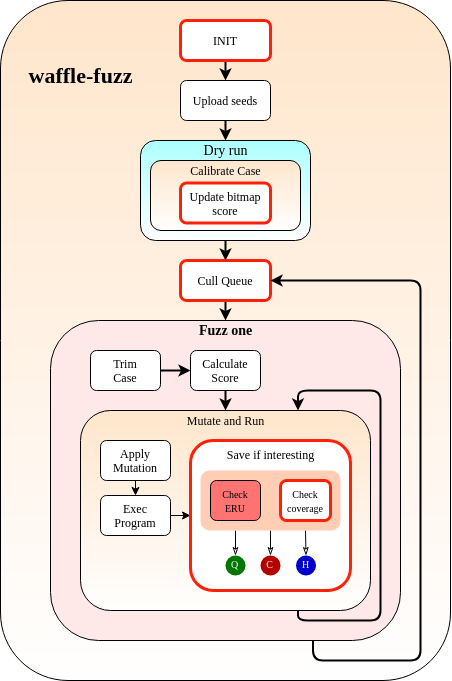
\includegraphics[width=0.8\textwidth]{Chapter3/waffle-fuzz-proc.png}
  \centering
  \caption{Waffle fuzzer: The red rectangles specify the new or changed components.}
  \label{fig:waffle-fuzz-proc}
\end{figure}

Waffle follows the same fuzzing procedure with modifications in processing the inputs and selecting next inputs to fuzz. As illustrated in Figure \ref{fig:waffle-fuzz-proc}, Waffle initializes the procedure by introducing new variables to the entries of the queue, as well as the changes to the \texttt{top\_rated} array of entries. After uploading the seeds, the fuzzing loop starts by culling the queue, modifying the priorities of the entries based on their execution features, i.e. the coverage and performance features, and finally starts fuzzing the next entry of queue. While calibrating the case, Waffle changes the bitmap scores (tracked by \texttt{top\_rated}s), and let's the fuzzer to considers the winners of the coverage test and performance tests. Before entering the mutation phase, Waffle calculates the score for havoc stage and trims the input as much as it can. The mutation methods are the same as it was in AFL. After each mutation, Waffle executes the program with the mutated input and collects the execution's info. These data are then processed and the features are extracted for the guidance. Waffle first checks if there is a new coverage, and then examines the info for new ERU's in execution. The mutation continues in deterministic and non-deterministic stages, and then the fuzzer continues with the next entry after culling the queue. As an overview, the rectangles with red boundries are the modified modules, and the module for checking ERU is added to the system.

% -T: Explain the data structures used and developed for fuzzing

Besides the initial configurations for starting a fuzz testing, Waffle adds a new shared memory to the system. \texttt{trace\_ERU} is an array in which each cell represents the ERU of an edge - or more than one edge, in case of collisions. The shared memory is then passed to the program for execution, and before each execution, it is cleared of any prior information. The structure of \texttt{queue\_entry}'s is changed by adding a new variable (i.e. \texttt{TERU}) for tracking the total ERU after execution of entry. In addition, the \texttt{top\_rated} array for tracking the winners of each edge is extended to maintain both the coverage and the performance winners (Figure \ref{fig:waffle-top_rated}). To track the performance measurements, Waffle first checks if an edge is in the coverage map, and then processes the performance info, and if a more resource exhaustive value is retrieved of execution, the second cell of the according index points to the winner \texttt{queue\_entry}. 

\begin{figure}[!b]
  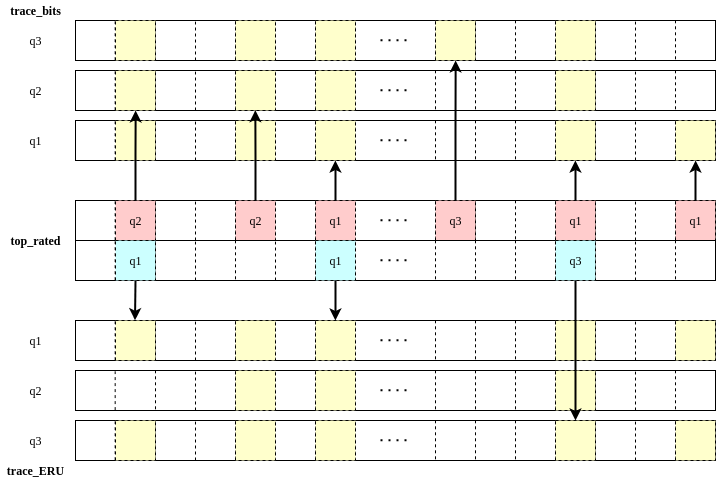
\includegraphics[width=0.8\textwidth]{Chapter3/waffle-top_rated.png}
  \centering
  \caption{\texttt{top\_rated} array: Waffle keeps track of the relevant coverage and performance features}
  \label{fig:waffle-top_rated}
\end{figure}

% -T: Dry run, Calibrate case, update bitmap score

Before starting the fuzzing loop, Waffle performs a dry run on the uploaded seeds to define an initial overview of the program; each execution fills the according \texttt{top\_rated[]}'s indices with the entries with a highest score. This score is based on two main factors: i) the \texttt{fav\_factor} of the execution as it was in AFL, and ii) maximizing the TERU of the corresponding execution. To investigate these execution's info, Waffle understands the paths and ERUs through the \textit{caliberation} of each test case. Waffle utilizes \texttt{update\_bitmap\_score} function with the power to analyze the new performance feature (i.e. ERUs) to update the information about the current state of queue entries \ref{lst:wafl-update-score}. The sparsness of the shared memories (\texttt{trace\_bits[]} and \texttt{ERUs[]}), and an expectation based on the fact that the repitition of same edges increases the TERU of execution, it is suitable to check the \texttt{var\_bytes[]} array, an array specifying the edges with variable number of visitation in an execution (Line 13). Briefly speaking, Waffle stores the pointer to the current entry of queue (i.e. $i_{th}$ index) in \texttt{top\_rated}, if it shows a higher TERU, the second index of the \texttt{top\_rated[i]} is assigned to this entry, else, it updates the first index for explaining a faster (and a smaller input size) execution \ref{fig:waffle-top_rated}. When the score is evaluated and the fitness of the entries are evaluated based on the information stored in \texttt{top\_rated}, the calibration phase continues, and Waffle stores the results for future use - that is when it culls the queue in the next step.

\lstinputlisting[language=C,style=CodeStyle,float=tb,label={lst:wafl-update-score},caption={\texttt{update\_bitmap\_score}: Waffle ignores the fav\_factor in case of a long lasting execution}]{Codes/Chapter3/waffle-fuzz/update_bitmap_score.c}

% -T: Cull queue

The generated queue of entries is checked to assign the priorities of the entries. The order of the entries in queue does not change, but Waffle (as AFL does) assignes the favorness of entries by comparing them based on the current state of the fuzzing. In another words, each element of the queue is analyzed, and if it \textit{looks} like a favorite entry, it is tagged as favorite, and else, it is marked as redundant and is ignored on it's turn to process. While processing the \texttt{top\_rated} entries, if an entry shows new coverage, it is tagged as favorite, otherwise, if it has is showing a \textit{different} ERU, the entry is tagged as the one selected for its \textit{class}. The classes of ERUs is based on integer value of the logarithm of its value, that is:

\begin{equation}
  \label{eq:eru-class}
  ERU\_class = \lfloor \lg(eru) \rfloor  
\end{equation}

which indicates the position of the leftmost bit in the integeral representation of ERU. The classes are used to remove the edges of the same class, and as a result, each edge is processes maximum of 32 times (for 32bit ERU integers). The outcome of the for loop on \texttt{top\_rated} holds the values of 0, for being not favored, 1 for being favored, and 2 to specify an entry representing its class. Yet, as Waffle is trying to increase the resource exhaustion, by iterating over the list of entries, we select the class and its representative entry with the highest ERU and change its favored value to 1. The rest of the entries with $favored == 2$ are set to redundant ($ favored \leftarrow 0 $). An snippet of the code is shown in Listing \ref{lst:cull-queue}.

\lstinputlisting[language=C,style=CodeStyle,label={lst:cull-queue},caption={Waffle \texttt{cull\_queue}}]{Codes/Chapter3/waffle-fuzz/cull_queue.c}

% -T: Fuzz one

The first favored entry of the queue is selected for fuzzing. First, Waffle keeps the \textit{trimming} procedure same as AFL's, and does not consider the changes in the \texttt{ERUs[]}. This is because of the fact that the trimming procedure maintains the values of the \texttt{trace\_bits[]} to remain the same, which their changes also modifies the cells of \texttt{ERUs[]}. Before the mutation loop, Waffle determines the effort it wants to take for the current case, and calculates \texttt{perf\_score} for this purpose.

% -T: Mutation (not modified), Execution

In both deterministic and havoc stages of mutation, fuzzer executes the program on new files and stores them if they expose interesting information. An input is interesting if i) it generates an input based on the heuristics for guidance to generate corrupted executions, ii) a crash is occured, or iii) a hang is occured. The results in (ii) and (iii) does not need any modification. Waffle generates inputs and examines them to verify if they show a \textit{new coverage}, or they are exhaustive. The main goals of Waffle are to guide the code coverage to grow, as well as generating resource exhaustive executions. Listing \ref{algo:waffle-save-if-interesting} presents a pseudocode of \textit{save\_if\_interesting}. 

\begin{algorithm}
    \KwIn{\textbf{$in-memory test case$}}
    CALL has\_new\_bits RETURNING hnb\;
    \textcolor{green}{CALL has\_better\_elite RETURNING hbe}\;
    \If{hnb or hbe}{
        SAVE case to file\;
    } 
    \caption{save\_if\_interesting}
    \label{algo:ifi-waffle}
\end{algorithm}
